\documentclass[twocolumn]{article}
\usepackage{xeCJK}
%\setCJKmainfont{IPAゴシック}
\setCJKmainfont{IPA明朝}
\usepackage[a4paper, top=1in, bottom=1in, left=2cm, right=2cm]{geometry}
\usepackage[singlespacing]{setspace}
\usepackage{amsmath}
\usepackage{amssymb}
\usepackage{graphicx}
\usepackage{hyperref}
\title{平板境界による屈折像からのアストロイドの再発見}  % タイトルを日本語に
\author{M. Ryu \\ {\href{mailto:mingshey@hafs.hs.kr}{mingshey@hafs.hs.kr}}}
\begin{document}
%\begin{japanese}
\renewcommand{\figurename}{図}
	\maketitle
	
	\section{はじめに}
	
	水に部分的に浸漬された鉛筆が曲がったように見える現象は、屈折の学習において一般的に最初に遭遇する身近な現象である。しかしながら、鉛筆の先端の見かけ上の位置は常に一定ではなく、観察角度によって変化することが観察される。鉛直上方から観察した場合の深さは初歩的な物理学の授業で取り扱われるが、斜め方向から観察した場合の深さや見かけ上の位置の変化については、深く掘り下げられることは少ない。おそらく、この現象は複雑であると考えられ、深く考察することが避けられているためであろう。実際、高度な光学の教科書においても、この単純な疑問は、レンズや曲面鏡などのより重要なトピックに埋もれてしまうことが多い。
	
	にもかかわらず、一見単純でありながら興味深いこの疑問は、研究者の好奇心を絶えず刺激する。筆者だけでなく、この疑問について考察した研究者も存在すると考えられる。本研究は、この疑問に対する解答を提供することを目的とする。

\section{概要}

読者の便宜のために、ここで簡潔に結論を示す。水中にある点状の物体について考える。観測点(POV)は水面上に位置する。物体とPOVは共通の法平面上に存在する。

物体とPOVを含む法平面を$xy$平面とし、法平面と水面の交線を$x$軸、物体を通る法線を$y$軸とする。

図\ref{fig:squashed_astroid}より、POVが法平面内で移動すると、物体の見かけの位置が変化する。これらの見かけの位置の軌跡は曲線を形成し、これは一種の(caustic) である\footnote{これは虚像の軌跡であるため、\textit{虚(virtual caustic)}と呼ぶことができる。}。

この曲線は「扁平化したアストロイド(squashed astroid)」であり、以下の式で表されることが示される。

$$ \left| \dfrac{x}{M} \right| ^ {2/3} + \left| \dfrac{y}{N} \right| ^ {2/3} = 1,$$

ここで、
$M = D/\sqrt{n^2 - 1}$ は全反射臨界角によって決定される入射距離の最大値を表し、
$N = D/n$ は真上から観察した場合の見かけの深さを表し、
$D$ は物体の実際の深さ、
$n$ は空気に対する水の屈折率である。

\begin{figure}
	\centering
	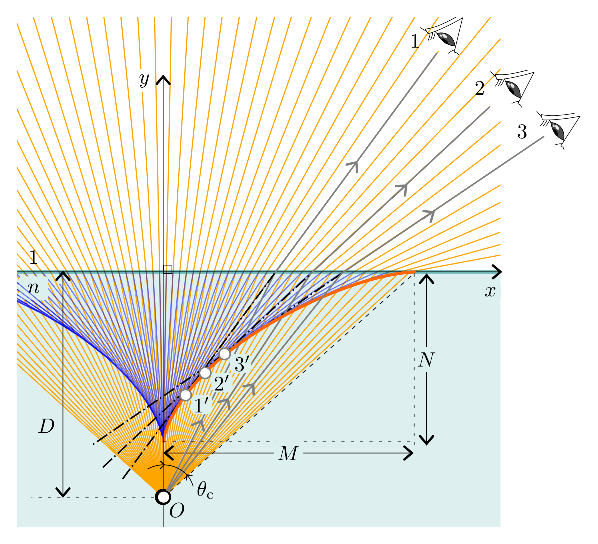
\includegraphics[width=2.7in]{g409.eps}
	\caption{像の軌跡}
	\label{fig:squashed_astroid}
\end{figure}

\section{公式の導出}

空気と水の屈折率をそれぞれ $n_1$ および $n_2$ とする。点状の物体 O は空気と水の界面から深度 D の位置にある。物体 O から発せられた光線は、界面上の点 A に入射する。点 A は $y$ 軸から距離 $\alpha$ に位置し、入射角は法線に対して $\theta_2$ である。この光線は界面で屈折し、空気中では同じ法線に対して $\theta_1$ の角度を持つ。

\begin{figure}
	\centering
	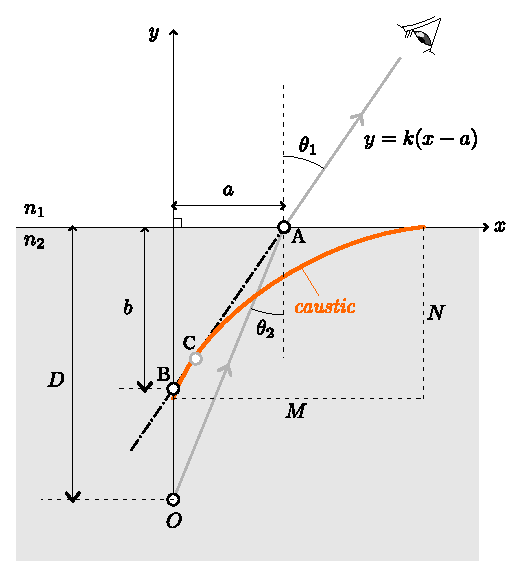
\includegraphics[width=3in]{g237.eps}
	\caption{空気-水の界面における光の屈折の幾何学的な関係}
	\label{fig:caustic}
\end{figure}

スネルの法則より、以下が成り立つ。
$$ \sin\theta_1 = \frac{n_2}{n_1} \sin\theta_2 = n\sin\theta_2.$$
屈折光線の延長線は次の式で表される。
$$y=k(x-\alpha),$$
ここで、
$$k=\dfrac{1}{\tan\theta_1}=\dfrac{\cos\theta_1}{\sin\theta_1},$$
であり、スネルの法則を考慮すると、
$$k=\dfrac{\sqrt{1-n^2\sin^2\theta_2}}{n\sin\theta_2}.$$

この直線は $y$ 軸上で点 B ($y=\beta$) と交わるため、
$$\beta = -k\alpha.$$

図\ref{fig:caustic}より、以下の関係が得られる。
$$\alpha = D\tan\theta_2 = \dfrac{D\sin\theta_2}{\cos\theta_2},$$
および
$$\begin{aligned}
	\beta &= -k\alpha \\
	&= -\dfrac{D\sin\theta_2}{\cos\theta_2}
	\dfrac{\sqrt{1-n^2\sin^2\theta_2}}{n\sin\theta_2}\\
	&=-\dfrac{D\sqrt{1-n^2\sin^2\theta_2}}{n\cos\theta_2}.
\end{aligned}$$

ここで、$K=\alpha/M$ および $H=\beta/N$ とおく。すると、
$$ \begin{aligned}
	K^2 + H^2 &= \dfrac{\alpha^2}{M^2}+\dfrac{\beta^2}{N^2}\\
	&=\dfrac{\left(n^2-1\right)\sin^2\theta_2 + 1-n^2\sin^2\theta_2}
	{\cos^2\theta_2}\\
	&=\dfrac{1-\sin^2\theta_2}{\cos^2\theta_2}\\
	&=1
\end{aligned}$$

ここで、無次元パラメータ $\xi=x/M$ および $\eta=y/N$ を導入する。 
$xy$ 平面上で視点 (POV) が移動すると、それに伴い、 
物体空間における点 $\mathrm{A}(\alpha, 0)$ および $\mathrm{B}(0, \beta)$ はそれぞれ、 
$\xi\eta$ 平面上の点 $\mathrm{K}(K, 0)$ および $\mathrm{H}(0, H)$ に変換される。 
重要な点として、これらの変換された点間の距離は、視点の移動によらず常に 1 に維持される。

図\ref{fig:astroid}に示すように、$\xi\eta$ 平面上で線分 $\overline{\mathrm{KH}}$ の軌跡は、アストロイド(astroid)と呼ばれるよく知られた幾何学的形状を形成する\footnote{「小惑星」を意味する アステロイド と混同しないこと} 
アストロイドは、以下の式で表される。
$$ \left| \xi \right|^{2/3} + \left| \eta \right|^{2/3} = 1 $$

\begin{figure}
	\centering
	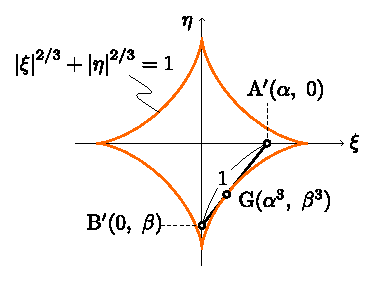
\includegraphics{g107.eps}
	\caption{$\xi\eta$平面における幾何学的な図}
	\label{fig:astroid}
\end{figure}

物体像は、$xy$ 平面上の 線分 $\overline{\mathrm{AB}}$と との接点 C に位置する。 
これは、隣接する光線束の発散点である。 
$\xi\eta$ 平面における対応する点は $\mathrm{G}(K^3, H^3)$ である。

したがって、像の座標 $(x_{\mathrm{C}}^{}, y_{\mathrm{C}}^{})$ は、次の関係式から求められる。
$$ \left\{ 
\begin{aligned}
	\xi_{\mathrm{G}}^{} &= \dfrac{x_{\mathrm{C}}^{}}{M} = K^3 = \dfrac{\alpha^3}{M^3},\\
	\eta_{\mathrm{G}}^{} &= \dfrac{y_{\mathrm{C}}^{}}{N} = H^3 = \dfrac{\beta^3}{N^3}.
\end{aligned}
\right.$$

すなわち、
$$ \left\{ 
\begin{aligned}
	x_{\mathrm{C}}^{} &= \dfrac{\alpha^3}{M^2},\\
	y_{\mathrm{C}}^{} &= \dfrac{\beta^3}{N^2}=-\dfrac{k^3\alpha^3}{N^2}.
\end{aligned}
\right.$$

ここで、
$$\sin\theta_2 = \dfrac{\alpha}{\sqrt{D^2+\alpha^2}},$$
を用いると、
$$k = \dfrac{\sqrt{D^2-(n^2-1)\alpha^2}}{n\alpha},$$
となり、像の位置をパラメータ $\alpha$ の関数として導出することができる。
$$ \left\{ 
\begin{aligned}
	x_{\mathrm{C}}^{} &= (n^2-1)\dfrac{\alpha^3}{D^2},\\
	y_{\mathrm{C}}^{} &= -\dfrac{n^2}{D^2}\dfrac{\alpha^3}{n^3\alpha^3}\left\{ D^2-(n^2-1)\alpha^2 \right\}^{3/2}\\
	&=-\dfrac{D}{n}\left\{ 1-(n^2-1)\dfrac{\alpha^2}{D^2} \right\}^{3/2}.
\end{aligned}
\right.$$

\section{水中の観測点}

物体の高さが $D$ で,空気と水の境界となる平面界面の上方にあり,観測点 (POV) が水中に没している場合,相対屈折率は 1 より小さくなります (すなわち,$1/n < 1$)。同様の論理により,以下のの式を導出することができます。

$$ \left| \xi \right|^{2/3} - \left| \eta \right|^{2/3} = -1, $$

ここで,$\xi = \dfrac{x}{W},$ $\eta = \dfrac{y}{Z},$ $W = \dfrac{nD}{\sqrt{n^2-1}},$ $Z = nD$ です。この曲線は,傾きが $\pm Z/W = \pm \sqrt{n^2-1}$ の漸近線を持ちます。

その結果,水中から見上げる上空の \emph{空景 (skyscape)} の像は,全反射の臨界角  で制限された円領域 (あるいはより正確には円錐) に圧縮されます (スネルの窓と呼ばれる)。この円形の広角ビューは,水中観察者から見ると,魚眼レンズで撮影した視野に似ています。

著者の知る限りでは,この曲線の形状を示す特定の名称は文献に確立されていません。この曲線の一般化された形式である

$$ \left| \xi \right|^{2/3} - \left| \eta \right|^{2/3} = \pm1, $$

は,水面上にある点光源から発せられた光線が屈折して水中で集まる様子を表すとして物理的な意味を持ち,また楕円と双曲線の関係に似てアストロイドとの関係があることを考えると,\emph{双曲アストロイド (hyperastroid)} という用語が適切な命名法として提案されます。(図\ref{fig:hyperastroid})

\begin{figure}
	\centering
	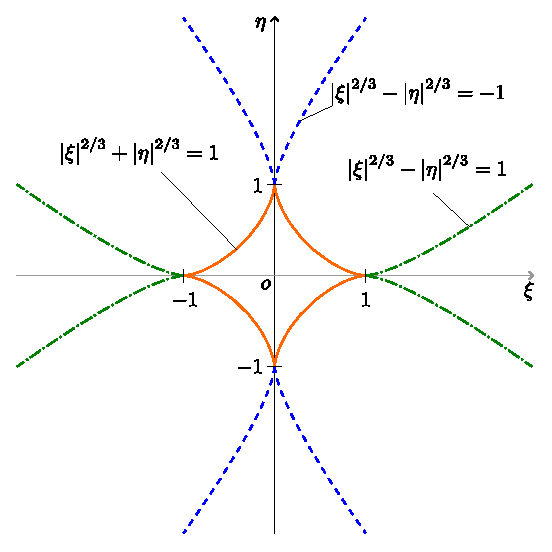
\includegraphics[width=3in]{g254.eps}
	\caption{アストロイドと双曲アストロイド}
	\label{fig:hyperastroid}
\end{figure}

アストロイドは \href{https://mathworld.wolfram.com/Astroid.html}{超楕円 (superellipse)} と呼ばれる曲線族に属しており,以下のように定義されます。

$$ \left| \xi \right|^{r} + \left| \eta \right|^{r} = 1. $$

アストロイドは $r = 2/3$ の場合です。

以下の式で定義される曲線の族は、\href{http://dynamicmathematicslearning.com/super-ellipse.html}{DML}\footnote{\ttfamily{dynamicmathematicslearning.com/super-ellipse.html}}において「スーパーハイパーボラ」と呼ばれている。

$$
\left| \xi \right|^{r} - \left| \eta \right|^{r} = \pm 1,
$$

\href{https://old.nationalcurvebank.org/superconicncb/superconicncb.htm}{NCB}\footnote{\ttfamily{nationalcurvebank.org/superconicncb/superconicncb.htm}}では、これらを総称して「スーパーコニック」と呼んでいるが、他の文献でこれらの用語を見つけることができず、これらの用語が分野内で確立された用語であるかどうかは不明である。

\section{像の検出}

閉形式の曲線を得ることができたので、物体と観測点の位置関係から像の位置を求めることができる。

\begin{figure}[h]
	\centering
	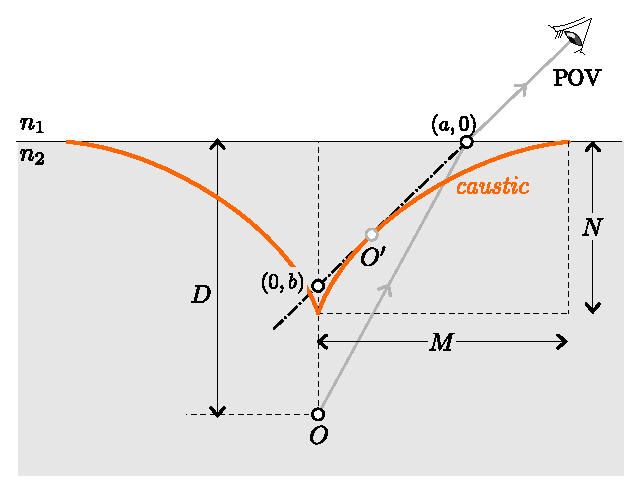
\includegraphics[width=3in]{g394.eps}
	\caption{曲線と物体からの光線の経路}
	\label{fig:caustic_raypath}
\end{figure}

観測点から曲線に接線を引く。この接点こそが、点光源の像の位置を表す。同時に、この接線が水面上と交わる点が入射点となり、物体から出た光線が屈折した地点を示す。

物体自体が水面下に広がっている場合でも、物体表面上の各点について同様に接線を引くことで像を求めることができる。物体表面を点が無断に移動しながら求めた像の軌跡が、物体全体の像となる。

\begin{figure}[h]
	\centering
	\includegraphics*[width=3in]{g240.eps}
	\caption{物体全体の像 (近似的な手法による)}
	\label{fig:extended_image}
\end{figure}

しかしながら、解析的に曲線への接線を引くことは困難であり、実際問題としては数値計算による近似解を求めるにとどまる。

別の方法としては、フェルマーの原理を用いて物体と観測点を結ぶ光路を数値的に求め、光線が水面上と交わる点の座標をもとに、アストロイドの接点を求める公式を利用して像の位置を求めることができる。Python による実装例は、\href{https://github.com/mingshey/python_projects/blob/main/Refraction_Image_en.ipynb}{github.com/mingshey/python\_projects} で公開されている。

\appendix
\newcommand{\pardiff}[2]{{\frac{\partial #1}{\partial #2}}}
\newcommand{\ilpardiff}[2]{{{\partial #1}/{\partial #2}}}
\section*{付録: アストロイドを包絡線として導出する}
直交座標系において、x軸上の点$(K, 0)$とy軸上の点$(0, H)$が常に距離aを維持しながら移動すると仮定する。このとき、$K^2+H^2=a^2$であり、ある瞬間における線分を含む直線の式は以下のように表される。
$$y=-\dfrac{H}{K}(x-K)$$
ここで、$H=\pm \sqrt{a^2-K^2}$を用いると、
$$y(x, K) = \mp \dfrac{\sqrt{a^2-K^2}}{K}(x-K)$$
となる。
Kの値が変化すると、2点を結ぶ線分または直線も変化し、その包絡線は各瞬間における停留点の軌跡、すなわち$\ilpardiff{y}{K} = 0$を満たす点の軌跡となる。この条件を満たす$(x, y)$を求めよう。

$$ \begin{aligned}
	\pardiff{y}{K} &= \pm\left[\left( \dfrac{1}{\sqrt{a^2-K^2}}+\dfrac{\sqrt{a^2-K^2}}{K^2}\right) (x-K) + \dfrac{\sqrt{a^2-K^2}}{K} \right]\\
	&= \pm \dfrac{(K^2+a^2-K^2)(x-K)+K(a^2-K^2)}{K^2\sqrt{a^2-K^2}}\\
	&= \pm \dfrac{a^2 x - K^3}{K^2 \sqrt{a^2 - K^2}}\\
	&= 0.
\end{aligned}
$$
したがって、停留点のx座標は $x = K^3/a^2$であり、そのy座標は

$$ \begin{aligned}
	y(x, K) &= \mp \dfrac{\sqrt{a^2-K^2}}{K}\left(\dfrac{K^3}{a^2}-K\right)\\
	& = \pm \dfrac{\left( a^2- K^2 \right)^{3/2}}{a^2}\\
	& = \dfrac{H^3}{a^2}
\end{aligned}
$$
となる。したがって、停留点の座標$(x, y)$は次の式を満たす。
$$ \left|\dfrac{x}{a}\right|^{2/3} + \left|\dfrac{y}{a}\right|^{2/3} = 1. $$
$\blacksquare$

%\end{japanese}
\end{document}